\documentclass{article}

\usepackage{amsmath}
\usepackage{amsfonts} % For math fonts.
\usepackage{amssymb} % For other math symbols not covered by amsmath.
\usepackage[pdftex]{graphicx} % For pictures, use \includegraphics[scale=decimal]{pic.png}; must be a .png file type.
\usepackage{multicol}
\usepackage{textcomp}
\usepackage[colorlinks = true, urlcolor = blue]{hyperref}
\usepackage{enumitem}
\usepackage{graphbox} 
\usepackage{subfig}
\usepackage{multicol}

\newcommand{\tab}{\hspace*{0.25in}}
\newcommand{\csq}[1]{\reflectbox{''}#1''}  %This produces CS style quotes.


\usepackage{tikz}
\usetikzlibrary{positioning, calc}
\usetikzlibrary{shapes.geometric,angles,quotes}


\usepackage{fullpage}
\usepackage{listings}
\lstset
{ %Formatting for code in appendix
    language=Python,
    basicstyle=\footnotesize,
    numbers=left,
    stepnumber=1,
    showstringspaces=false,
    tabsize=2,
    breaklines=true,
    breakatwhitespace=false,
}


\begin{document}


\begin{flushright}
Selection Statements\end{flushright}

\vspace*{-1.5em}
\noindent\makebox[\linewidth]{\rule{\paperwidth}{0.4pt}}


\vspace*{2em}

\begin{enumerate}

%start_of_questions

%new_question
	\item 
		Use the following code to answer the below questions\\
		\mbox{ \hspace*{0.25in}	\lstinputlisting[language=Python]{./code/c1.py}}
		\begin{enumerate}
			\item Find four values of my\_var so each of the four assignment statements will be executed: 
				each value should cause one assignment statement to be executed.
			\item Find four ranges of my\_var values that will cause each of the four assignment 
				statements to be executed.
		\end{enumerate}


%new_question
	\item 
		In your own words, describe the difference in logic of the following two sets of code:\\
		\begin{minipage}{.5\textwidth}
			(a) \mbox{\hspace*{2em} \lstinputlisting[language=Python]{./code/c2a.py}}
		\end{minipage}
		\begin{minipage}{.5\textwidth}
			(b) \mbox{\hspace*{2em} \lstinputlisting[language=Python]{./code/c2b.py}}
		\end{minipage}


%new_question
	\item
		When driving in a car and approaching a traffic control light, \textit{green} means go, 
		\textit{yellow} means yield, and \textit{red} means stop.  Assuming there is a variable 
		named \textit{light\_color}, write a program that prints either the word \textit{go}, 
		\textit{yield}, or \textit{stop} depending of the value of \textit{light\_color}.  
		Let the user input the value of \textit{light\_color}.


%new_question
	\item 
		The table below show what your resting heart rate should be based on age and athleticism.  
		Write a program that asks the user their age and desired athleticism goal, and then outputs 
		what their resting heart rate should be.

		\begin{minipage}{.45\textwidth}
			\begin{tabular}{c|cc}
				& \multicolumn{2}{c}{Athleticism}\\
				Age & Above Average & Below Average \\ \hline
				20 -- 39 & 47 -- 72 & 73 -- 93\\
				40 -- 59 & 46 -- 71 & 72 -- 94\\
				60 -- 79 & 45 -- 70 & 71 -- 97 \\
			\end{tabular}
		\end{minipage}
		\begin{minipage}{.45\textwidth}
			\vspace*{1em}
			Your end output should look similar to this
			\fbox{\parbox{\textwidth}{ Enter your age: 45\\
			Enter your athleticism goal: Below Average\\
			Your resting heart rate should be between 72--94.}}
		\end{minipage}


%new_question
	\item 
		Write a program that prompts the user to enter three integers and displays the integers 
		in increasing order (smallest to largest).  You may not use the built-in functions 
		\textit{max}(), \textit{min}(), \textit{sort}() or \textit{sorted}().


%new_question
	\item 
		Write a program that prompts the user to enter three integers and displays the integers 
		in decreasing order (largest to smallest).  You may not use the built-in functions 
		\textit{max}(), \textit{min}(), \textit{sort}() or \textit{sorted}().


%new_question
	\item 
		In Harry Potter, the currency consists of knuts, sickle, and galleon.  There are 29 knuts in 
		one sickle and 17 sickles in one galleon.  Write a program that will convert some amount of 
		knuts into the fewest amount of coins possible.  Only print non-zero values, meaning don't print 
		something similar to ``0 sickles.''  For example,
		\begin{itemize}
			\item Given 32 knuts, output 1 sickle 3 knuts
			\item Given 544 knuts, output 1 galleon 4 sickles 18 knuts
			\item Given 993 knuts, output 2 galleons 7 knuts. 
				Do \textbf{not} output 2 galleons 0 sickle 7 knuts.
		\end{itemize}



%new_question
	\item
		Write a program that asks the user for three numbers, and then determines (and outputs) which of the 
		numbers is the largest.  Do not use the built-in function \textit{max}().\\
		For example, \\ \ \hfill
		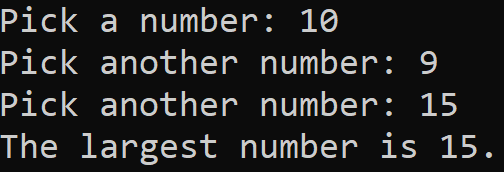
\includegraphics[height = 0.6in]{./imgs/largest_ex1.PNG} \hfill
		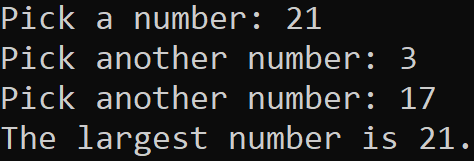
\includegraphics[height = 0.6in]{./imgs/largest_ex2.PNG} \hfill \ 
		%{C:/Users/cd7926ej/OneDrive - MNSCU/CIS121/Question Generator/2_expressions/Texted/imgs/largest_ex1.PNG}



%new_question
	\item
		Write a program that asks the user for three numbers, and then determines (and outputs) which of the 
		numbers is the smallest.  Do not use the built-in function \textit{min}().\\
		For example, \\ \ \hfill
		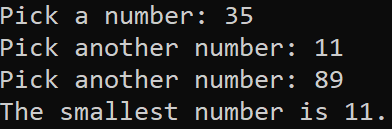
\includegraphics[height = 0.6in]{./imgs/smallest_ex1.PNG} \hfill
		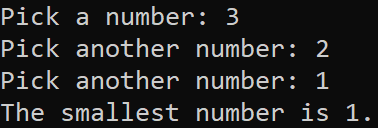
\includegraphics[height = 0.6in]{./imgs/smallest_ex2.PNG} \hfill \ 




%new_question
	\item		
		The table below shows the maximum health of characters based on race and class for a new video game 
		I am creating.  Write a program that asks the user for the race and the class of their character, 
		and then sets the \textit{health\_points}	variable according to the table below.
		\begin{flushright}
		\begin{tabular}{c|cc}
			& \multicolumn{2}{c}{Race}\\
			Class & Elf & Ogre \\ \hline
			Warrior & 150 & 200\\
			Bard & 75 & 100\\
			Wizard & 25 & 50 \\
		\end{tabular}
		\end{flushright}
		
		\vspace*{-6em}
		\textit{health\_points} = -1\\
		\#Your code here.
		\vspace*{3em}		
		%\begin{tabular}{|ll}
		%	\\			
		%	\textit{health\_points} = -1 \\[5pt]
		%	\#Your code here. \\[5pt]
		%	& \\ & \\ & \\ & \\ & \\ & \\ & \\ & \\ & \\ & \\ & \\ & \\ & \\ & \\ & \\ & \\ & \\
		%	& \\ & \\ & \\ & \\ & \\ & \\ & \\ & \\ & \\ & \\
		%\end{tabular}


%new_question
	\item 
		(Game: heads or tails)  Write a program that lets the user guess whether the flip of a coin 
		results in heads or tails.  The program randomly generates an integer 0 or 1, which 
		represents head or tail.  The program prompts the user to enter a guess and reports whether 
		the guess is correct or incorrect.\\
		Hint: These should be your first two lines of code.
		\begin{verbatim}
		    from random import randint
		    value = randint(0,1) #picks a random integer. Either 0 or 1.
		\end{verbatim}



%new_question
	\item 
		%https://edabit.com/challenge/b8wRDMWgMZTN2nmfx
		Ask the user for three integers.  Determine (and output) how many copies of the same number 
		the user entered.\\
		For example, \\ \ \hfill
		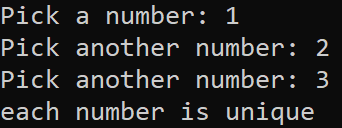
\includegraphics[height = 0.6in]{./imgs/uniqueIntCount1.PNG} \hfill
		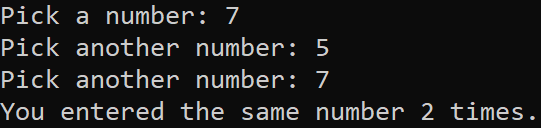
\includegraphics[height = 0.6in]{./imgs/uniqueIntCount2.PNG} \hfill \ 

	
%new_question
	\item 
		Primary U.S. interstate highways are numbered 1-99.  Odd numbers (like 5 or 95) go north/
		south, and evens (like 10 or 82) go east/west.  Auxiliary highways are numbered 100-999, and 
		service the primary highway indicated by the rightmost two digits.  Thus, I-405 services 
		I-5, and I-290 services I-90.
		
		Note: 200 is not a valid auxiliary highway because 00 is not a valid primary highway 
		number.\\
		
		Let the user pick a highway number.  Given a valid highway number, indicate whether it runs 
		north/south or east/west.  If it is an invalid highway number, indicate that it is an 
		invalid highway number. \\
		For example,
		
		\hfill
		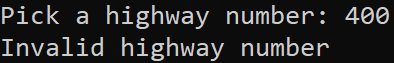
\includegraphics[width = 2in]{./imgs/highwayValidator1.PNG} \hfill
		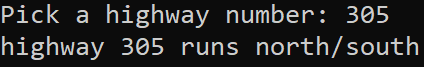
\includegraphics[width = 2in]{./imgs/highwayValidator2.PNG} \hfill \ 

		\hfill 
		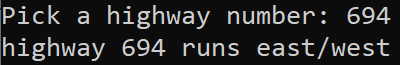
\includegraphics[width = 2in]{./imgs/highwayValidator3.PNG} \hfill 
		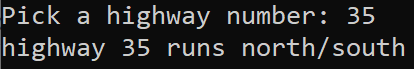
\includegraphics[width = 2in]{./imgs/highwayValidator4.PNG} \hfill \ 


%new_question
	\item 
		Write a program that prompts the user for a letter and checks whether the letter is a vowel 
		or consonant.  A vowel should output \textit{\csq{vowel}}, and a consonant should output 
		\textit{consonant}.  You may assume only lower case letters. Below is sample output.\\
		Hint: In the English language, a, e, i, o, and u are the vowels.
	
		\begin{figure}[h]
		\centering
			\begin{minipage}{.5\textwidth}
			\centering
				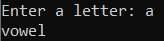
\includegraphics[scale=1.2]{./imgs/vowelYesAlt.png}
			\end{minipage}%
				%
			\begin{minipage}{.5\textwidth}
			\centering
				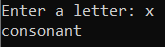
\includegraphics[scale=1.1]{./imgs/vowelNoAlt.png}
			\end{minipage}
		\end{figure}



%new_question
	\item 
		The table below shows what time different age groups (by grade) can swim at the pool.  There 
		are two time options, morning and afternoon.  Write a program that asks the user their grade 
		and whether they'd like to go in the morning or afternoon, and outputs the time the pool is 
		available for them.

		\begin{minipage}{.45\textwidth}
		\begin{tabular}{c|cc}
						& \multicolumn{2}{c}{Pool times}\\
			Grade 		& Morning 	& Afternoon \\ \hline
			k, 1 -- 3 	& 9 AM 		& 1 PM\\
			4 -- 8 		& 10 AM 	& 2 PM\\
			9 -- 12 	& 11 AM 	& 3 PM \\
		\end{tabular}
		\end{minipage}
		%
		\begin{minipage}{.45\textwidth}
			\ \\
			Your end output should look similar to this
			%(if you were to actually run the code).

			\fbox{\parbox{\textwidth}{ Enter your grade: 5\\
			Enter Morning OR Afternoon: Morning\\
			The pool is open at 10 AM.}}
		\end{minipage}




%new_question
	\item 
		At the local ice cream store they have 3 flavors, which are Vanilla, Chocolate, and Strawberry.  
		Write a program that ask the user which type of ice cream they want and print the flavor they 
		selected.  However, if they picked a flavor that is not available, inform the user of such.
	
		\hfill 
		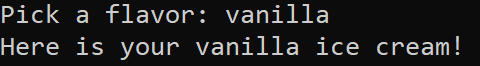
\includegraphics[width = 2.5in]{./imgs/iceCreamFlavors1.PNG} \hfill 
		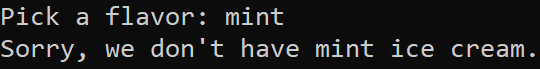
\includegraphics[width = 2.5in]{./imgs/iceCreamFlavors2.PNG} \hfill \ 


%new_question
	\item 
		%https://edabit.com/challenge/sfqudQHQ3HPpd7dZb
		Create a game of Rock, Paper, Scissors that takes user inputs.  
		The first input should be player 1 and the second 
		input should be player 2.  Print the winner according to the following rules. 
		\begin{itemize}
			\item Rock beats Scissors
			\item Scissors beats Paper
			\item Paper beats Rock
		\end{itemize}		
		For example:

		\hfill 
		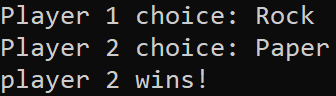
\includegraphics[height = 0.5in]{./imgs/RockPaperScissors1.PNG} \hfill 
		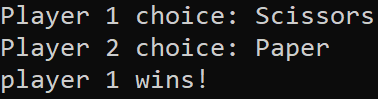
\includegraphics[height = 0.5in]{./imgs/RockPaperScissors2.PNG} \hfill  
		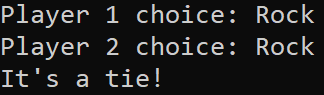
\includegraphics[height = 0.5in]{./imgs/RockPaperScissors3.PNG} \hfill \ 


%new_question
	\item 
		%https://edabit.com/challenge/ancAxGEF9MsLWXDqe
		Write a program that asks the user for three side lengths of a triangle, and prints 
		the type of triangle.  The types of triangles are 
		\begin{itemize}
			\item No sides equal: \csq{scalene}
			\item Two sides equal: \csq{isosceles}
			\item All sides equal: \csq{equilateral}	
		\end{itemize}
		For example:

		\hfill 
		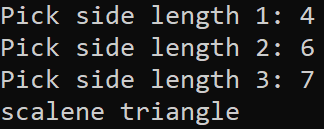
\includegraphics[height = 0.7in]{./imgs/typeOfTriangle1.PNG} \hfill 
		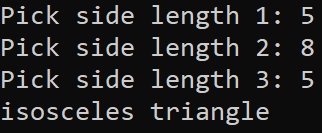
\includegraphics[height = 0.7in]{./imgs/typeOfTriangle2.PNG} \hfill  
		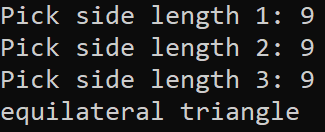
\includegraphics[height = 0.7in]{./imgs/typeOfTriangle3.PNG} \hfill \ 



%new_question
	\item 
		%https://edabit.com/challenge/8pDH2SRutPoaQghgc
		Luke Skywalker has friends and family, but he is getting older and having trouble 
		remembering them all.  Write a program that Luke (the user) can input a name and it 
		outputs the relation defined in the table below.
		\begin{center}
		\begin{tabular}{|l|l|} \hline
			Person 		& Relation \\ \hline \hline
			Darth Vader	& Father \\ \hline
			Leia		& Sister \\ \hline
			Han			& Brother in law\\ \hline
			R2D2		& Droid \\ \hline
		\end{tabular}\\ \hspace*{1in} *If he types any other name, report \csq{unknown}.
		\end{center}
		


%end_of_questions


%\item Write a program that will convert some amount of pennies into the fewest amount of dollars and coins possible.  For example, 75 pennies is 3 quarters.  86 pennies is 3 quarters, 1 dime, and 1 penny.  130 pennies is 1 dollar, 1 quarter and 1 nickel.  Let the user pick the number of pennies.  You may assume the largest input is 499 pennies.\\
%Hint: the way to do this is to always substitute for the largest denomination if available.  For example, if there is at least 100 pennies substitute for a dollar before quarters.

\end{enumerate}
\end{document}




%new_question
	\item 
		%https://edabit.com/challenge/sfqudQHQ3HPpd7dZb









